\documentclass[12pt,a4paper]{article}
\usepackage[T2A]{fontenc}
\usepackage[utf8x]{inputenc}
\usepackage[english,russian]{babel}
\usepackage{amsmath,amsfonts,amssymb,amsthm,mathtools}

\author{Коллективный разум}
\title{\textit{Бе}се\textit{ды} с \textit{Ба}тю\textit{шкой}}
\date{\today}

\begin{document}

\maketitle
\newpage

\section*{Гомеоморфизм}

Пусть $M,N \subset \mathbb{R}^{n}.$ $f:M\longrightarrow N$ -- отображение\footnote{Отображение $f:M\rightarrow N$ -- закон, который каждому элементу $x \in M$ ставит в  соответствие единственный элемент $y \in N.$}.\\


Отображение $f$ \textbf{непрерывно в точке $a$}, тогда и только тогда, когда 
		\[\lim_{x \to a}{f(x)} = f(a)\]

\textbf{Непрерывность по Коши:}
	\[ 
		\forall \varepsilon > 0 ~
		\exists \delta_{\varepsilon} > 0: ~
		(\forall x\in U_{\delta_{\varepsilon}}(a)\cap M
		\Rightarrow f(x)\in U_{\varepsilon}(f(a))) 
	\]
\begin{center}
	или в многомерном случае
\end{center}
	\[
		\forall \varepsilon > 0	~
		\exists \delta_{\varepsilon} > 0:
		(\forall x\in B_{\delta_{\varepsilon}}(a)
		\Rightarrow \rho(f(x),f(a))<\varepsilon),
		\footnote{
			Здесь ~
			$B_{\delta_{\varepsilon}} = 
			\{y\in \mathbb{R}^n | ~ \rho(y,a) <
			\delta_{\varepsilon}\}$,
			а ~
			$\rho(x,y) = \sqrt{\sum_{i=1}^n(x_i - y_i)^2}$
				}
	\]	
	
	
	\textbf{По Гейне:}
		\[ \forall  x_n \to a \Rightarrow f(x_n) \to f(a) \]\\
	
	\textbf{\large{Определение:}} отображение $f:M \to N$ называется \underline{\textbf{гомеоморфизмом}}, если
	\begin{itemize}
		\item $f$ -- биекция,
		\item $f$ -- непрерывна,
		\item $f^{-1}$ -- непрерывна
	\end{itemize}
	Говорят, что $M$ гомеоморфно $N$ и обозначается
	\begin{center}
	$M \cong N$
	\end{center}
	
	
	
	\textbf{\large{Упражнение 1:}} доказать или опровергнуть, что ллюбая нерпрерывная биекция является гомеоморфизмом.
	
	\textbf{\large{Упражнение 2:}} доказать, что 
	\begin{center}
	$(0,1) \cong  \mathbb{R}$
	\end{center}	
	
	\textbf{\large{Упражнение 2:}} доказать, что 
	\begin{center}
	D =$\{(x,y)\in \mathbb{R}^2 | x^2 + y^2 < 1\}$ 
	\newline $D\cong \mathbb{R}^2$ 
	\end{center}
	\newpage
\section*{Многообразие}

Пусть \(M \subset \mathbb{R}^n\) такое, что \(\exists k\in \mathbb{N}\), 
\( \forall \varepsilon >0\):
\begin{center}
 либо \(U_{\varepsilon} (x)\cap M \cong \mathbb{R}^k\)
\end{center}
\begin{center}
 либо \(U_{\varepsilon} (x)\cap M \cong \mathbb{R}_{+}^k\)
\end{center}
где \(\mathbb{R}_{+}^k = \{(x_1,x_2,...,x_k)| x_1,..., x_{k-1} \in \mathbb{R}, x_k\ge 0\}\)
\newline в этом случае M является \underline{\textbf{многообразием}} размерности k.
\newline Если \(\nexists\) окрестности \(U_{\varepsilon} (x): U_{\varepsilon} (x)\cap M \cong \mathbb{R}^k\), то \(x\) - \textbf{граничная точка}, иначе \(х\)- \textbf{внутренняя точка}.
\newline Если множество граничных точек пустое (\(\emptyset\)), то \(M\)- многообразие \textbf{без края}, в противном случае \textbf{с краем}.
\newline \textbf{Примеры:}
\newline 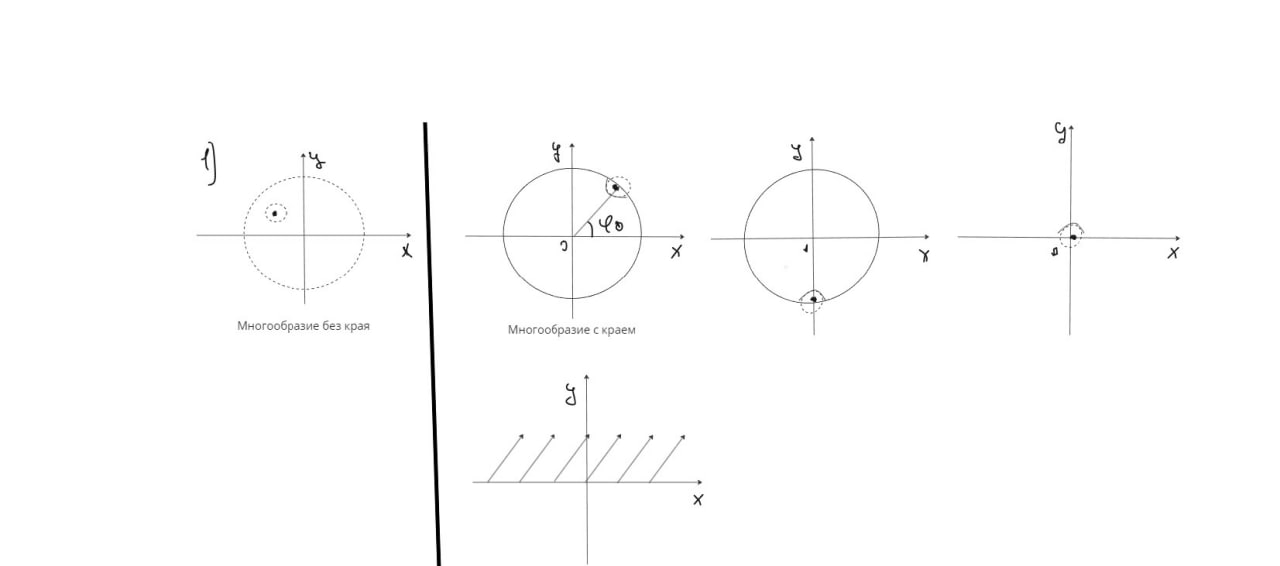
\includegraphics[scale=0.7]{image1.jpg}
\newline 2. Окружность: \(S^1 = \{(x,y)\in \mathbb{R}^2| x^2 + y^2 =1\}\) 
\newline 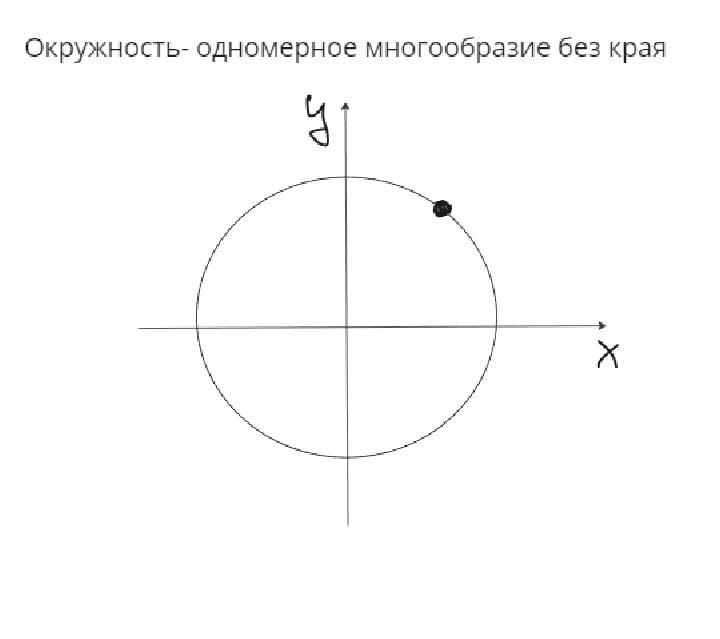
\includegraphics[scale=0.85]{image2.jpg}
\newpage 3. Сфера: \(S^2 = \{(x,y,z)\in\mathbb{R}^3| x^2+y^2+z^2=1\}\)
\newline 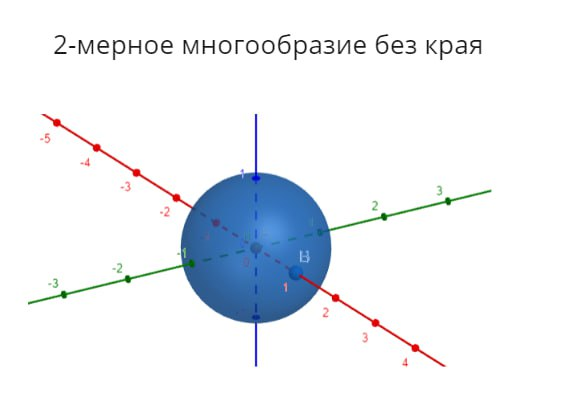
\includegraphics[scale=0.5]{image3.jpg}
\newline 4. Тор. Рассматриваем как поворот единичной окружности вокруг оси Oz.
\(T=\{(x,y,z)\in \mathbb{R}^3\)|
\begin{equation*}
\begin{cases}
(y - 2)^2 + z^2=1
\\
x =0
\end{cases}
\end{equation*}
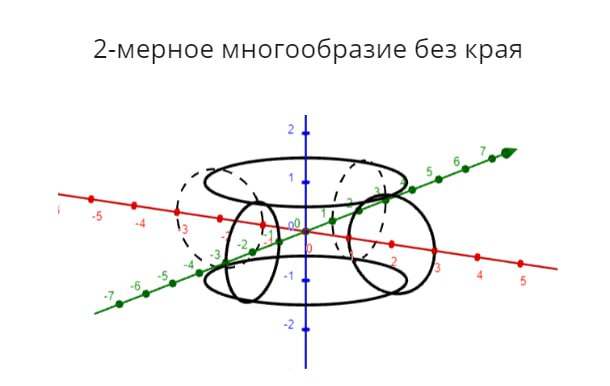
\includegraphics[scale=0.5]{image4.jpg}
\newpage 5. Цилиндр.
\newline \(C = \{(x,y,z)\in \mathbb{R}^3\)|
\begin{equation*}
\begin{cases}
x^2+y^2=1
\\
0\leq z\leq1 
\end{cases}
\end{equation*}
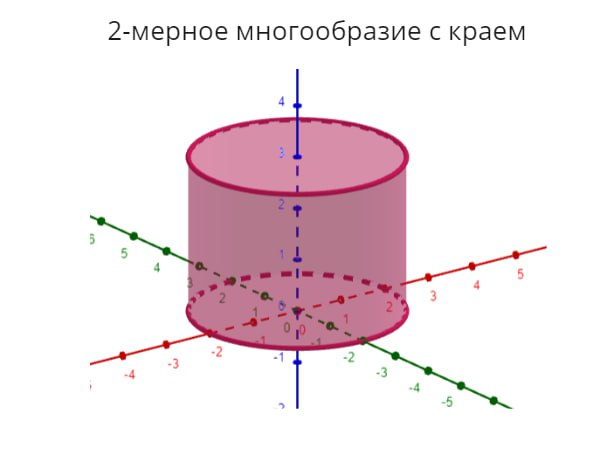
\includegraphics[scale=0.5]{image5.jpg}

    
    
	
		



	
	
	
	







\end{document}

